% ISBI 2027 - randomized benchmark-exposure study for chest X-ray encoders. Build: latexmk -pdf main.tex
% Numbers in the results come from scripts (tables/*.tex, numbers.tex); never type them by hand.
\documentclass{article}
\usepackage{spconf,amsmath,graphicx,booktabs,xcolor}
\usepackage[hyphens]{url}
\usepackage{enumitem}
\setlist{nosep, leftmargin=14pt}
\newcommand{\todo}[1]{\textcolor{red}{[#1]}}
% Generated by scripts/make_paper_numbers.py from results/ and data/. Do not edit by hand.
\newcommand{\NFrontal}{79{,}543}
\newcommand{\NPatients}{26{,}982}
\newcommand{\NB}{25{,}014}
\newcommand{\NPbase}{15{,}000}
\newcommand{\NPclean}{15{,}002}
\newcommand{\NHa}{4{,}013}
\newcommand{\NHb}{4{,}000}
\newcommand{\NEThree}{6{,}000}
\newcommand{\NEFifteen}{6{,}001}
\newcommand{\NEHundred}{4{,}006}
\newcommand{\NEFiveHundred}{507}
\newcommand{\EFiveHundredPatients}{184}
\newcommand{\AgeRange}{60--61}
\newcommand{\APRange}{84--86}
\newcommand{\FemaleLarger}{39--43}
\newcommand{\FemaleEFiveHundred}{53}
\newcommand{\PrevSpread}{3}
\newcommand{\ViewShareHigh}{56}
\newcommand{\RadNIHShare}{3}
\newcommand{\StepsOne}{18{,}160}
\newcommand{\StepsTwo}{18{,}171}
\newcommand{\AdaptOneStart}{0.712}
\newcommand{\AdaptOneEnd}{0.748}
\newcommand{\KnnOneStart}{0.629}
\newcommand{\KnnOneEnd}{0.655}
\newcommand{\PosCtlOne}{0.557}
\newcommand{\AdaptTwoStart}{0.704}
\newcommand{\AdaptTwoEnd}{0.744}
\newcommand{\KnnTwoStart}{0.633}
\newcommand{\KnnTwoEnd}{0.657}
\newcommand{\PosCtlTwo}{0.553}
\newcommand{\ExtN}{518}
\newcommand{\ExtTrainN}{6{,}000}
\newcommand{\ExtProxy}{0.804}
\newcommand{\ExtProxyCI}{0.778--0.828}
\newcommand{\ExtRad}{0.813}
\newcommand{\ExtRadCI}{0.790--0.836}
\newcommand{\ExtInit}{0.763}
\newcommand{\MarginPts}{0.5}
\newcommand{\HolmM}{67}
\newcommand{\LowRange}{$-0.20$ to 0.74}
\newcommand{\LowCIMax}{2.0}
\newcommand{\EFiveHundredRunGap}{2.8}
\newcommand{\HbRunGap}{0.1}
\newcommand{\PrimDelta}{$-0.42$}
\newcommand{\PrimCI}{$-0.83$ to $-0.01$}
\newcommand{\PrimBootCI}{$-1.01$ to 0.16}
\newcommand{\PrimP}{0.092}
\newcommand{\CleanDelta}{$-0.37$}
\newcommand{\CleanCI}{$-0.72$ to $-0.01$}
\newcommand{\CleanBootCI}{$-0.94$ to 0.18}
\newcommand{\CleanP}{0.090}
\newcommand{\UoneDelta}{$-0.18$}
\newcommand{\UoneCI}{$-0.51$ to 0.15}
\newcommand{\UoneBootCI}{$-0.69$ to 0.31}
\newcommand{\UoneP}{0.38}
\newcommand{\LLDrop}{0.020}
\newcommand{\LLDropClean}{0.040}
\newcommand{\LLDropUone}{0.022}
\newcommand{\LLCI}{0.009--0.031}
\newcommand{\LLBootCI}{0.002--0.039}
\newcommand{\LLP}{$<$0.001}
\newcommand{\LLHolm}{0.019}
\newcommand{\MatchedDelta}{$-0.45$}
\newcommand{\MatchedCI}{$-0.88$ to $-0.01$}
\newcommand{\UnpairedHundredOne}{$-1.25$}
\newcommand{\UnpairedHundredTwo}{0.63}
\newcommand{\EHundredHarder}{1.7}
\newcommand{\EFiveHundredOne}{$-7.24$}
\newcommand{\EFiveHundredOneCI}{$-11.16$ to $-2.86$}
\newcommand{\EFiveHundredOneDrop}{7.2}
\newcommand{\EFiveHundredOneAdjDrop}{7.1}
\newcommand{\EFiveHundredOneHolm}{0.043}
\newcommand{\EFiveHundredTwo}{$-3.97$}
\newcommand{\EFiveHundredTwoCI}{$-7.82$ to $-0.03$}
\newcommand{\EFiveHundredTwoDrop}{4.0}
\newcommand{\EFiveHundredTwoAdjDrop}{4.6}
\newcommand{\EFiveHundredTwoHolm}{1}
\newcommand{\AuditorRange}{0.52--0.56}
\newcommand{\AuditorMax}{0.56}
\newcommand{\CEHundred}{0.61}
\newcommand{\CEFiveHundred}{0.78}
\newcommand{\TwinOne}{0.65}
\newcommand{\TwinOneTPR}{3.4}
\newcommand{\TwinTwo}{0.64}
\newcommand{\TwinTwoTPR}{4.0}
\newcommand{\HeadThree}{0.51}
\newcommand{\HeadFifteen}{0.53}
\newcommand{\HeadHundred}{0.61}
\newcommand{\HeadFiveHundred}{0.78}
\newcommand{\NullInvOne}{0.51}
\newcommand{\NullHeadOne}{0.51}
\newcommand{\NullInvTwo}{0.52}
\newcommand{\NullHeadTwo}{0.50}
\newcommand{\HeadTPRHundred}{2.4}
\newcommand{\HeadTPRFiveHundred}{11.1}
\newcommand{\NMembers}{202}
\newcommand{\NNonmembers}{518}
\newcommand{\GateAUC}{0.52}
\newcommand{\GateCI}{0.47--0.57}
\newcommand{\RadBackbone}{0.48}
\newcommand{\RadBackboneCI}{0.43--0.53}
\newcommand{\MDE}{0.567}
\newcommand{\RadHead}{0.72}
\newcommand{\RadHeadCI}{0.67--0.75}
\newcommand{\SizeWidth}{0.55}
\newcommand{\SizeHeight}{0.55}
\newcommand{\ModalAUC}{0.71}
\newcommand{\ModalCI}{0.66--0.76}
\newcommand{\ModalMembers}{134}
\newcommand{\ModalNonmembers}{321}
\newcommand{\RadHeadLow}{0.71}
\newcommand{\RadHeadLowCI}{0.67--0.75}
\newcommand{\IntensityAUC}{0.48}
\newcommand{\LabelsAUC}{0.52}
\newcommand{\CtlOne}{0.53}
\newcommand{\CtlOneCI}{0.48--0.58}
\newcommand{\DiffOne}{0.19}
\newcommand{\DiffOneCI}{0.12--0.25}
\newcommand{\CtlTwo}{0.49}
\newcommand{\CtlTwoCI}{0.45--0.54}
\newcommand{\DiffTwo}{0.22}
\newcommand{\DiffTwoCI}{0.16--0.28}

\renewcommand{\dbltopfraction}{0.9}\renewcommand{\dblfloatpagefraction}{0.8}\setcounter{dbltopnumber}{2}
\title{Seen in pretraining: randomized exposure in chest X-ray encoders}
\name{Zhibin Wang}
\address{Academy of Artificial Intelligence and Advanced Technology\\Xi'an Jiaotong-Liverpool University, Taicang, China}
\begin{document}
\maketitle
\begin{abstract}
Chest X-ray encoders are often evaluated on benchmarks whose test images were in their pretraining data; RAD-DINO's released checkpoint saw each NIH ChestX-ray14 test image about 101 times. We randomized such exposure in two crossover runs of DINO pretraining of DINOv2-S on CheXpert, with patients assigned to arms seen 0 to 500 times. At dose 100, the pre-specified premium of seen over unseen test images in frozen-probe macro-AUC was \PrimDelta{} points (90\% CI \PrimCI), excluding a premium above $+\MarginPts$ points, though equivalence was not shown; with probes trained on equally exposed images it was \MatchedDelta{} (\MatchedCI; exploratory). Exposure was detectable from the DINO head (membership AUC \CEHundred) or against the other crossover run (\TwinTwo--\TwinOne), but barely from the backbone with its initial weights as reference (at most \AuditorMax). In exploratory analyses, RAD-DINO's released head separated the CheXpert validation images in its training list from test images (AUC \RadHead; pre-specified backbone score \RadBackbone; our encoders, which saw neither set, \CtlTwo--\CtlOne). Label-free exposure thus did not inflate frozen-probe AUC here, while a released head can reveal what data a model saw.
\end{abstract}
\begin{keywords}
chest X-ray, foundation models, self-supervised learning, benchmark contamination, membership inference
\end{keywords}

\section{Introduction}\label{sec:intro}
Chest X-ray foundation encoders are pretrained on hundreds of thousands of public radiographs, then evaluated with frozen features on public benchmarks that often share those images. Unusually, the public RAD-DINO checkpoint comes with the full list of its 882{,}775 training images~\cite{microsoft2024raddinocard}. The list contains all 112{,}120 NIH ChestX-ray14 images~\cite{wang2017chestxray8}, including the 25{,}596 official test images and all 30{,}000 images of RSNA Pneumonia~\cite{shih2019rsna}, a benchmark drawn from NIH that the RAD-DINO paper~\cite{perezgarcia2025raddino} lists as external although its model also pretrains on NIH (Sec.~2.1.1, Table~D.1). At the released checkpoint (step 35{,}000 of 100{,}000, 2{,}560 images per step~\cite{microsoft2024raddinocard}), each training image had been seen about 101 times on average. Other encoders show similar, often partial overlaps (Table~\ref{tab:audit}).

An image-only encoder never sees a diagnosis, so this exposure is not label leakage, but it may still raise benchmark scores. Self-supervised vision encoders memorize individual training images~\cite{meehan2023dejavu,wang2024sslmem}, yet the linear-probe train--test gap does not track this memorization~\cite{meehan2023dejavu}. Medical audits found source overlap between benchmarks and pretraining data~\cite{xu2026medvlm} and higher accuracy on patients shared across whole-slide benchmark splits~\cite{zhang2026wsileak}, but such comparisons cannot isolate exposure, because exposed and clean cases differ in other ways too. A controlled re-pretraining of single-cell models showed that membership signals grow with model capacity relative to data~\cite{ali2026scfm}. None of these studies randomizes label-free exposure to isolate its premium in an imaging encoder.

To measure it, we continue DINO pretraining~\cite{caron2021dino,oquab2024dinov2} of a small DINOv2 encoder, the proxy, on CheXpert~\cite{irvin2019chexpert}, with patients assigned at random to arms whose images are seen 0 to 500 times, and compare frozen-encoder probe AUC on exposed and held-out images (Fig.~\ref{fig:overview}). A crossover run exchanges the dose-100 arm with a held-out arm, so every image in the primary contrast is compared with itself. We also ask whether membership scores that a trainer or an outside auditor could compute detect exposure, and apply them to the released RAD-DINO. The analysis plan was hash-logged before training (not publicly registered); it is released with its amendments, deviations and all code at \url{https://github.com/shenfuqili/chexpert-exposure-isbi2027}.

\begin{figure*}[t]\centering
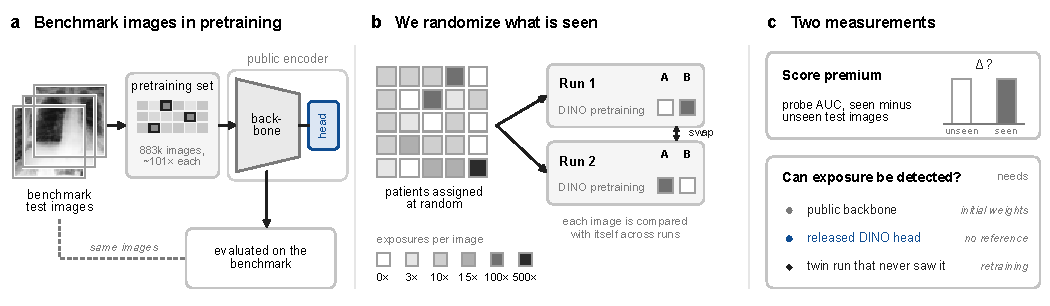
\includegraphics[width=\textwidth]{figures/fig1_overview.pdf}
\caption{Overview. (a) Encoders pretrained on collections that contain benchmark test images are evaluated on those benchmarks; RAD-DINO saw each of its training images about 101 times. (b) Patients are assigned at random to arms seen 0 to 500 times; a second run swaps arm A (H\textsubscript{a}) and arm B (E100). (c) We measure the probe-AUC premium and whether exposure is detectable.}\label{fig:overview}
\end{figure*}

\begin{table}[t]\centering\scriptsize\setlength{\tabcolsep}{2.4pt}
\caption{Benchmark exposure of public chest X-ray encoders. M: exposed, verified against a released manifest; S: exposed per stated training data; D: exposed via derivation (RSNA images are NIH images); p: partly (share if computable); St: only the source's training split used (not exposure); N: not a stated source; ?: unclear. $^*$ checked at image level; $^\dagger$ benchmark validation data selected or tuned the checkpoint; $^c$ Ark+ uses the VinDr test list for validation. RAD-DINO and Ark+ released image-level lists, so their rows are the most complete. Other NIH subsets follow the RSNA column; five other encoders show no documented exposure on these benchmarks. The full audit, with sources, is released. Benchmarks: NIH ChestX-ray14~\cite{wang2017chestxray8}, RSNA Pneumonia~\cite{shih2019rsna}, CheXpert (CX)~\cite{irvin2019chexpert}, MIMIC-CXR~\cite{johnson2019mimiccxr}, VinDr-CXR~\cite{nguyen2022vindrcxr}.}\label{tab:audit}
\begin{tabular}{lcccccc}
\toprule
Encoder & NIH & RSNA & CX val & CX test & MIMIC & VinDr \\
\midrule
RAD-DINO~\cite{perezgarcia2025raddino} & M & D$^*$$^\dagger$ & M & St$^*$ & St$^*$ & N$^*$$^\dagger$ \\
EVA-X~\cite{yao2025evax} & St & Dp$^*$\,{\tiny 63--73\%} & St & St & ? & N \\
MedImageInsight~\cite{codella2024medimageinsight} & Sp$^*$\,{\tiny 45.4\%} & Dp$^*$\,{\tiny 48.5\%} & N & N & St & N \\
ELIXR~\cite{xu2023elixr} & ? & Dp & N$^\dagger$ & N & St & N \\
CheXzero~\cite{tiu2022chexzero} & N & N & N$^\dagger$ & N & S & N \\
Ark{+}~\cite{ma2025arkplus} & St$^*$ & Dp$^*$\,{\tiny 89\%} & St$^*$ & St$^*$ & St$^*$ & St$^*$$^{c}$ \\
CXR-CLIP~\cite{you2023cxrclip} & ? & Dp\,{\tiny 59--80\%} & St$^\dagger$ & St & St & N \\
\bottomrule
\end{tabular}
\end{table}


\begin{figure*}[t]\centering
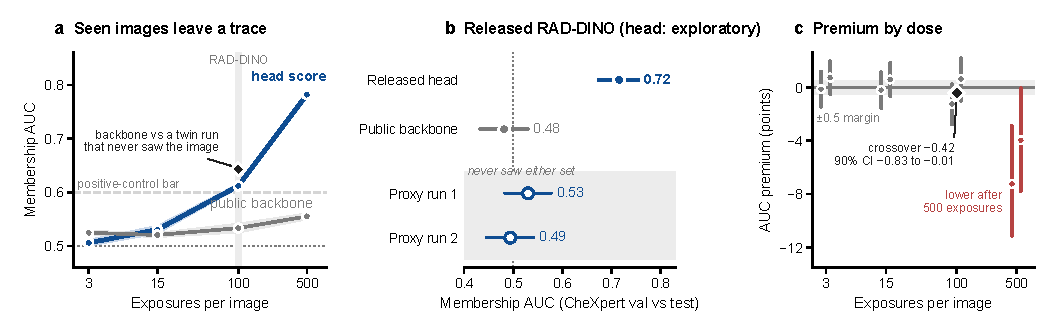
\includegraphics[width=\textwidth]{figures/fig2_main.pdf}
\caption{Exposure leaves a trace but, at dose 100, no premium above 0.5 AUC points. (a) Membership AUC of exposed arms vs H\textsubscript{b} (line, mean of two runs; band, range): blue, reference-free head score (exploratory); gray, backbone invariance minus the initial encoder's; black, the same against the twin run; dashed, positive-control bar; gray column, RAD-DINO's exposure. (b) RAD-DINO on its CheXpert validation images (in its training list, $n{=}202$) vs test images ($n{=}518$), proxy runs as controls; 95\% bootstrap CIs. (c) Unpaired premium in AUC points (95\% CIs; red, CI below zero) and the pre-specified crossover estimate (90\% CI); gray band, $\pm0.5$ margin.}\label{fig:main}
\end{figure*}

\section{Randomized exposure experiment}\label{sec:design}
\textbf{Arms.} We drew \NPatients{} patients at random from the downsampled CheXpert training split and assigned them, with all \NFrontal{} of their frontal images, to nine groups (seed fixed before download). A background set (\NB{} images) and the probe-training set P\textsubscript{base} (\NPbase) were seen 10 times; a second probe-training set P\textsubscript{clean} (\NPclean) and two held-out test arms, H\textsubscript{a} and H\textsubscript{b} (\NHa{} and \NHb), were never seen; test arms E3, E15, E100 and E500 (\NEThree, \NEFifteen, \NEHundred{} and \NEFiveHundred{} images) were seen 3, 15, 100 and 500 times, dose being the number of batches an image enters. The pre-specified estimand is thus the premium of exposing test images, with probes trained on images seen 10 times or never. Dose 100 matches RAD-DINO's average; E500 is the membership positive control. The larger arms were similar in age, AP share and label prevalence (within \PrevSpread{} points); E500 (\EFiveHundredPatients{} patients) had more women (\FemaleEFiveHundred\% vs \FemaleLarger\%).

\textbf{Encoder.} The proxy started from DINOv2-S/14~\cite{oquab2024dinov2} and continued DINO training (EMA teacher; two 224-pixel global and eight 98-pixel local crops; Sinkhorn--Knopp targets over 4{,}096 prototypes; no iBOT, unlike RAD-DINO). Its projection head used batch normalization and was trained alone for the first 10\% of steps, so the backbone saw about 90\% of each image's views. We used batch size 64 and RAD-DINO's schedules with the learning rate scaled by $\sqrt{64/1024}$. After the default settings collapsed in a pilot, these changes and a sweep on P\textsubscript{clean} that set DINOv2's KoLeo weight to 0 were fixed before the formal runs. The runs took \StepsOne{} and \StepsTwo{} steps (7\,h each on a laptop RTX~4050); Run~2 used a new seed and swapped H\textsubscript{a} and E100.

\textbf{Premium.} Frozen teacher CLS features of a center crop were extracted at the start, at 35\% of training (the stage of RAD-DINO's released checkpoint) and at the end. A one-vs-rest logistic probe trained on P\textsubscript{base}, tuned by patient-grouped cross-validation, gives the macro-AUC over the five CheXpert competition labels (uncertain labels negative). The primary endpoint is the crossover premium at dose 100,
\begin{equation}
\Delta_x=\tfrac12\big[(A^{(2)}_{G_1}-A^{(1)}_{G_1})+(A^{(1)}_{G_2}-A^{(2)}_{G_2})\big],
\end{equation}
where $G_1$ and $G_2$ are the images of H\textsubscript{a} and E100 and $A^{(r)}_G$ is their macro-AUC in run $r$; each bracket compares the same images exposed and unexposed, and the average cancels run differences. Its null variance comes from random image sets exposed equally in both runs (P\textsubscript{clean} and H\textsubscript{b}); we also report the patient bootstrap. Both are conditional on our two runs. Premiums are in AUC points (0.01 AUC); equivalence within $\pm\MarginPts$ points, the pre-specified smallest effect of interest, is tested with two one-sided tests at $\alpha=0.05$. Holm-corrected secondary endpoints (\HolmM{} tests) include the unpaired premium against the pooled never-seen arms at each dose and snapshot (bootstrap $p$-values, not the planned permutation test), a $k$-NN version, membership AUCs, and the primary contrast with a P\textsubscript{clean} probe, with uncertain labels positive, or in per-image label log-likelihood. An exploratory amendment trains the probes instead on images exposed as often as the test images, cross-fitted between patient halves of H\textsubscript{a} and of E100.

\textbf{Membership.} The pre-specified membership score is augmentation invariance, as in EncoderMI~\cite{liu2021encodermi}: the mean pairwise cosine similarity of CLS features over eight fixed augmented views, minus the same under a reference encoder, which is the twin run (the crossover partner, as in SSLMem~\cite{wang2024sslmem}) for E100 and H\textsubscript{a} and the initial encoder otherwise. A secondary score, the DINO loss under the run's own heads, is calibrated the same way. Exposed arms are compared with H\textsubscript{b}, the only test arm never seen in either run (the plan said H); E500 must exceed AUC 0.6 as the positive control.

\textbf{RAD-DINO.} RAD-DINO's manifest lists the 234 CheXpert validation images and none of the 668 test images (full-resolution copies from~\cite{saporta2022chexlocalize}, JPEG-encoded identically), a natural but non-randomized split into \NMembers{} member and \NNonmembers{} non-member frontal images. A DINOv2-B classifier must fail to separate them (patient-grouped AUC $<0.55$) before membership scores are compared. The pre-specified score is invariance under RAD-DINO minus that under DINOv2-B, its initialization (detectable AUC \MDE{} at 80\% power). Post hoc amendments, each written before its computation, add a reference-free head score (the negated mean cross-entropy between the head's outputs for pairs of views, also on proxy arms) and, after its RAD-DINO result, proxy controls, never-seen arm pairs and checks of size, fine detail, intensity and labels.

\section{Results}\label{sec:results}
\textbf{Validity.} Training adapted the encoder without collapse (held-out probe macro-AUC \AdaptOneStart{}$\to$\allowbreak\AdaptOneEnd{} and \AdaptTwoStart{}$\to$\allowbreak\AdaptTwoEnd; $k$-NN AUC also rose). On the CheXpert test set (\ExtN{} frontal images; unregistered) the Run-1 proxy reached \ExtProxy{} (95\% CI \ExtProxyCI), a competent encoder (RAD-DINO at 518 pixels: \ExtRad; initial DINOv2-S: \ExtInit).

\textbf{Premium.} At dose 100 the crossover premium was \PrimDelta{} points (90\% CI \PrimCI; $p=\PrimP$; Fig.~\ref{fig:main}c): a premium of $+\MarginPts$ is excluded, but the interval extends below $-\MarginPts$, so equivalence was not shown (the test had little power). The patient-bootstrap interval, wider in every crossover contrast, was \PrimBootCI{} (95\%). With 90\% CIs, a P\textsubscript{clean} probe gave \CleanDelta{} (\CleanCI), uncertain labels as positive \UoneDelta{} (\UoneCI), and probes cross-fitted within each arm, so that probe-training and test images were exposed equally, \MatchedDelta{} (\MatchedCI; exploratory). Per-image label log-likelihood fell by \LLDrop{} nats (95\% CI \LLCI; Holm $p=\LLHolm$), but not after Holm correction under bootstrap variance (\LLBootCI).

Doses 3 and 15 were uninformative (unpaired premiums \LowRange, 95\% CIs up to $+$\LowCIMax), and no contrast there or at 35\% of training survived correction. At dose 500 the premium was \EFiveHundredOne{} points in Run~1 (95\% CI \EFiveHundredOneCI; Holm $p=\EFiveHundredOneHolm$) and \EFiveHundredTwo{} in Run~2 (\EFiveHundredTwoCI; Holm $p=\EFiveHundredTwoHolm$). E500 is small and its AUC differed by \EFiveHundredRunGap{} points between runs at identical exposure (\HbRunGap{} for H\textsubscript{b}), so this drop is suggestive. The $k$-NN premium was never significant.

\textbf{Detection.} Detection depended on access (Fig.~\ref{fig:main}a). Backbone invariance with the initial encoder as reference, all an outside auditor has without retraining, gave only \AuditorRange{} at every dose (at dose 100 the pre-specified reference is the twin run), against \NullInvOne{} and \NullInvTwo{} for never-seen arm pairs (post hoc); it failed the positive control (E500: \PosCtlOne{} and \PosCtlTwo), which by the plan makes the membership analysis insensitive. Against the twin run the same score gave \TwinOne{} and \TwinTwo{} at dose 100. Head-based scores detected exposure: the pre-specified secondary score gave \CEHundred{} at dose 100 and \CEFiveHundred{} at dose 500, and the head score \HeadThree, \HeadFifteen, \HeadHundred{} and \HeadFiveHundred{} at doses 3 to 500 (unseen pairs, post hoc: \NullHeadOne{} and \NullHeadTwo). Single images were hard to identify: at 1\% false positives the head score flagged \HeadTPRHundred\% of dose-100 and \HeadTPRFiveHundred\% of dose-500 images.

\textbf{RAD-DINO.} The two sets passed the DINOv2-B gate (AUC \GateAUC, 95\% CI \GateCI), and the pre-specified backbone score did not separate them (\RadBackbone, \RadBackboneCI). RAD-DINO's released head did (\RadHead, \RadHeadCI; Fig.~\ref{fig:main}b), exceeding the head score of the two proxy runs, which saw neither set (\CtlOne{} and \CtlTwo), by \DiffOne{} (\DiffOneCI) and \DiffTwo{} (\DiffTwoCI). Image width, height, intensity statistics and labels barely separated the sets (AUC \SizeWidth, \SizeHeight, \IntensityAUC, \LabelsAUC), and the head score stayed at \ModalAUC{} within the most common image size and at \RadHeadLow{} (\RadHeadLowCI) after low-pass filtering to 224-pixel detail. These checks point to memorization, but they were written after the head result, and with non-randomized sets a remaining release difference cannot be excluded.

\section{Discussion}\label{sec:discussion}
In our proxy, test-image exposure at RAD-DINO's dose was detectable from the DINO head but did not raise frozen-probe AUC by more than 0.5 points, whether probes were trained on less-exposed or equally exposed images. The result omits report- or label-trained encoders and familiarity with a dataset's hospitals, scanners and case mix, which randomization holds equal and which keeps an overlapping benchmark from being external; we suggest calling such sets in-source.

An auditor with only the backbone and its initial weights saw a weak signal, near that of never-seen arms except at dose 500. The backbone score detected exposure clearly only against a model trained without the images, which an auditor would have to train, whereas the head score needed no reference, as D\'ej\`a vu's projector memorization suggests~\cite{meehan2023dejavu}. A released head therefore lets anyone check whether a model saw a benchmark; with private data it would also reveal membership, though weakly for single images. Despite a lower capacity-to-data ratio, RAD-DINO's head separated its training images better than our proxy's (\RadHead{} vs \HeadHundred{} at dose 100); a residual release difference could also explain this.

\textbf{Limitations.} The proxy is small (ViT-S, 224 pixels, batch 64, no iBOT or KoLeo) and was trained on one dataset; E100 and E500 supplied \ViewShareHigh\% of its training views, against about \RadNIHShare\% for NIH test images in RAD-DINO. We did not test fine-tuning, segmentation or checkpoint selection on benchmark data.

\section{Compliance with ethical standards}
This study used only public, de-identified data (CheXpert~\cite{irvin2019chexpert}, CheXlocalize~\cite{saporta2022chexlocalize}); ethical approval was not required, as confirmed by the license of the open-access data.

\section{Acknowledgments}
The author thanks the RAD-DINO authors for releasing the manifest and DINO head. This work received no funding, and the author declares no conflicts of interest. Code, figures, the exposure audit and the draft text were produced with Claude (Anthropic); the author checked all content and takes full responsibility for it.

\bibliographystyle{IEEEbib}
{\scriptsize\bibliography{refs}}
\end{document}
